\documentclass{beamer}
\usetheme{CambridgeUS}
\usecolortheme{beaver}
\title[Generative models for shape parametrization]{Generative models for shape parametrization}
\author[G. Padula]{\textbf{Guglielmo Padula}}
\institute{University of Trieste}

\date{}

\usepackage{graphicx}
\usepackage{tikz}
\usepackage{animate}
\usetikzlibrary{positioning,arrows.meta,quotes}
\usetikzlibrary{shapes,snakes}
\usetikzlibrary{bayesnet}
\tikzset{>=latex}
\tikzstyle{plate caption} = [caption, node distance=0, inner sep=0pt,
below left=5pt and 0pt of #1.south]
\begin{document}
\begin{frame}
\titlepage
\end{frame}

\begin{frame}{General Objective}
The general objective of our research is, given a set of 3D meshes generated by complex methods with a large number of parameters, to find a generative model such that:
\begin{itemize}
\item Reduces the number of effective parameters via dimensionality reduction
\item Sampling (and if possible training)  using this method should be fast as possible
\item Generated samples should satisfy some \textbf{convex} equality and/or inequality constraint   
\item (\textbf{Optional}) the distribution of useful quantities associated to the object should be similar between the generated samples and the real samples.
\end{itemize}
\end{frame}
\begin{frame}{Motivation}
\begin{itemize}
\item Complex methods are very computationally complex (the data generated in the code uses VFFD which is fast, howewer there are methods based on differential equations that take days to complete)
\item A possible application are inverse problems with non convex constraints, which require exaustive search,  they would scale exponentially in the number of parameters.
\item Ideally we would like to run simulation on this samples, and indeed to get not this simulations to explode, we need some convex constraints on the output. 
\end{itemize}
\end{frame}
\begin{frame}{Data}
We focus on the problem of deforming a naval hull bulb. The data is obtained by deforming using Volume Preserving FFD with 27 parameters, which deforms object by moving control points and preserves the volume. We want volume preservation because it is a nice property in simulations. It can be rewritten as a sequence of linear constraints. As we want to focus only on the bulb, we first take only one half of the ship, and then we do two cuts to obtain the bulb.  The ship is a triangular mesh so it has an internal topology.\\
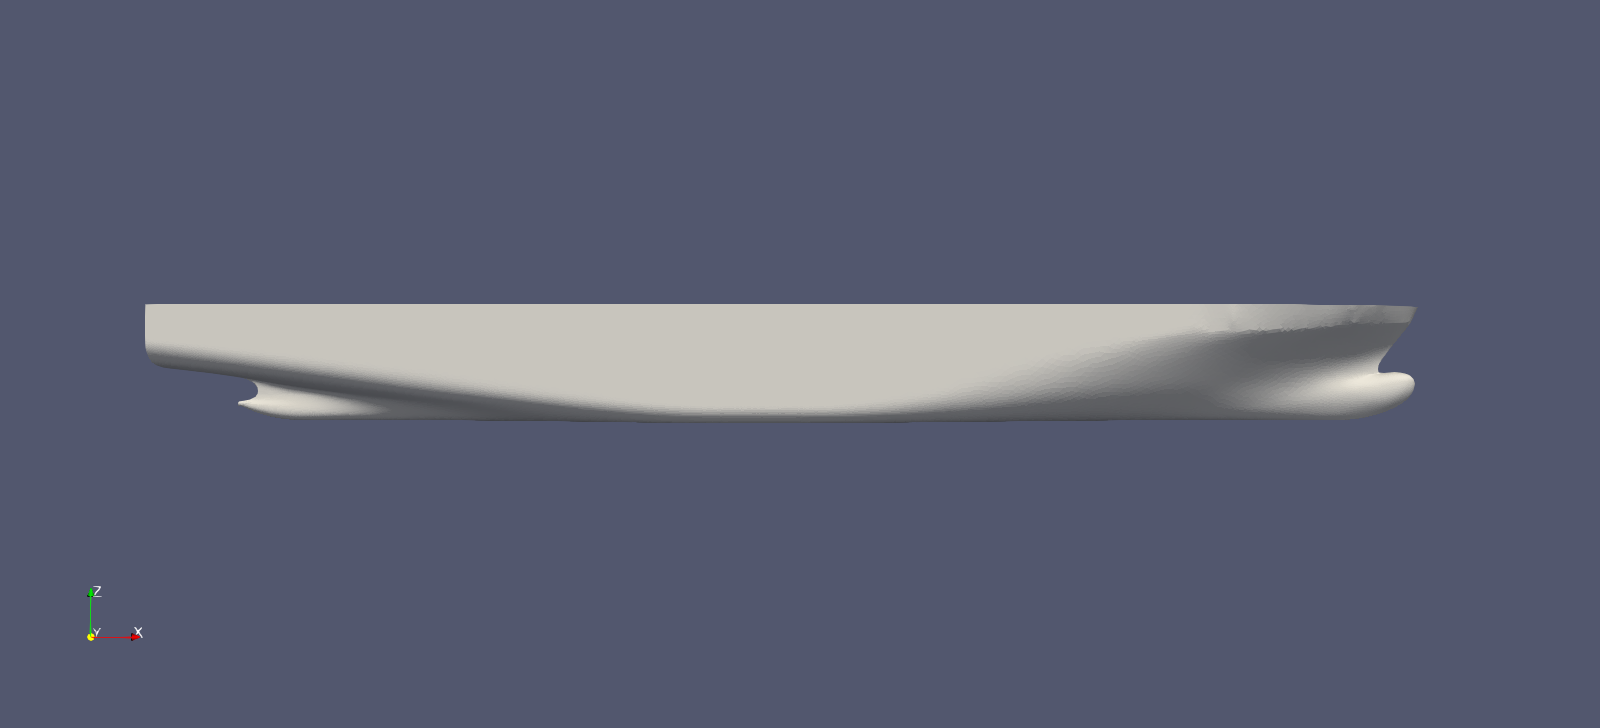
\includegraphics[scale=0.08]{naval}
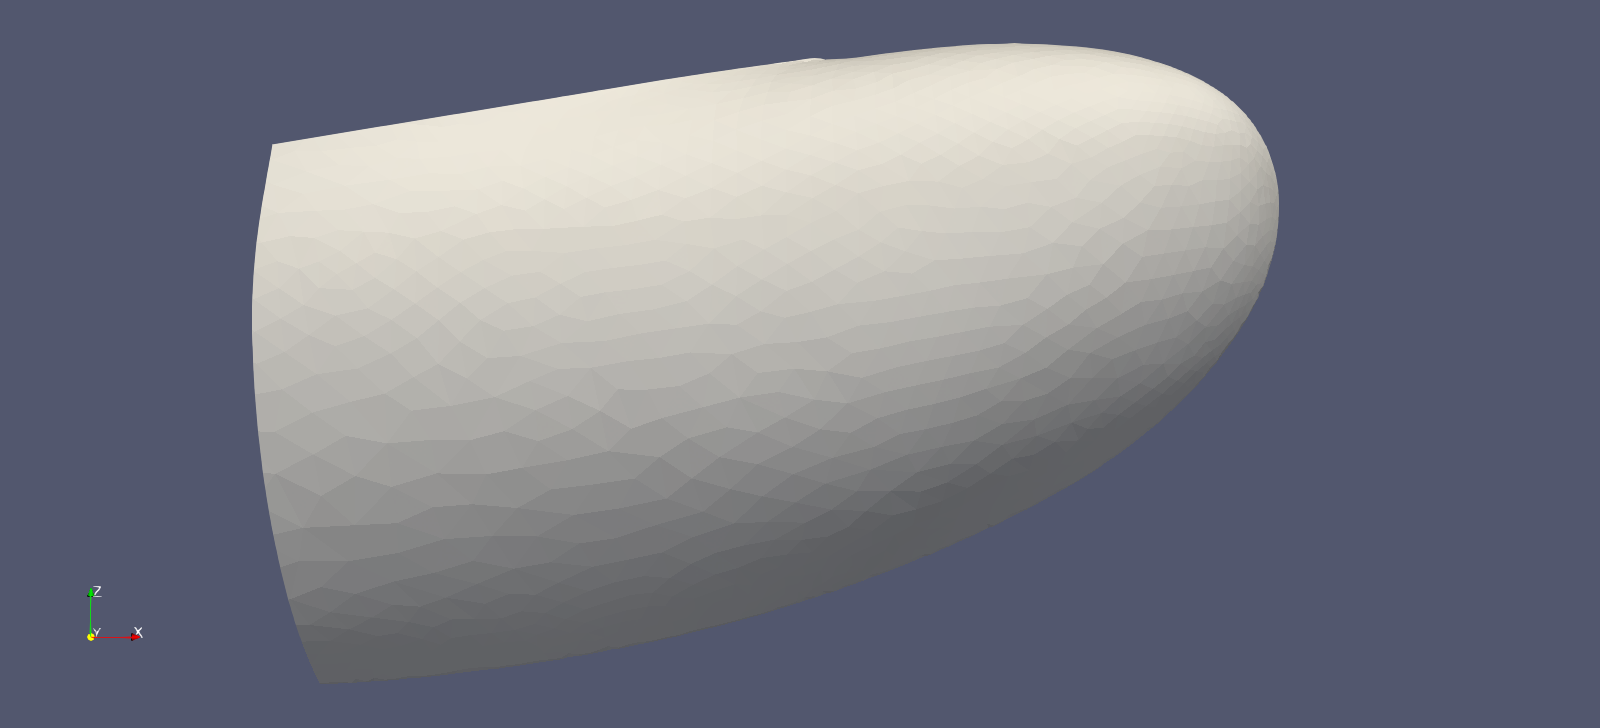
\includegraphics[scale=0.08]{bulbo}
\end{frame}
\begin{frame}{The generative models}
Our generative model should not touch the points on the boundary and move the points on the symmetry plane only horizontally. It should also preserve volume exactly. For this reason we need to heavely customize classic generative models and we split the data in two parts, a part ($x$) that will consist in the points that don't belong to the simmetry plane and a part $y$ that belong to the simmetry plane.
We use:
\begin{itemize}
\item Vanilla Autoencoder
\item Variational Autoencoder
\item Boundary Equilibrium GAN
\item Adversarial Autoencoder
\end{itemize}
All this models require an Encoder and a Decoder, whose architectures will be the same in every model.
All models are trained using AdamW.
\end{frame}
\begin{frame}{Long life to the LBR}
Our basic layer (which we call LBR) is formed with:
\begin{itemize}
\item A linear Layer
\item A BatchNorm1D Layer
\item A ReLU Layer
\item A Dropout Layer
\end{itemize}
\end{frame}
\begin{frame}{Custom Layers}
We also use a series of custom layer to improve the training and the sampling:
\begin{itemize}
\item A PCA Layer
\item A smoothing Layer
\item A volume normalization Layer
\end{itemize}
These layers are not strictly necessary to obtain decent samples in the generation phase (the network learns to preserve volume even without the layer), howewer the sample quality is greatly increased with the use of this layers.
\end{frame}
\begin{frame}{PCA Layer}
We use PCA to reduce the initial dimensionality of the data, which will consist in two layers: a PCATranformLayer and a PCAInverseTransformLayer. Note that PCA does not compress data as the relative reconstruction error is very low (around $10^{-8}$).
\end{frame}
\begin{frame}{Smoothing Layer}
This is a layer that applies laplacian smoothing $$K_{i}=\frac{1}{|N_{i}|}\sum_{j \in N_{i}} K_{j}$$ where $N_{i}$ are the neighbours of index $i$. Note that while $K_{i}$. Note that the laplacian smoother is applied only to points that are not on the boundary and on the simmetry plane. 
\end{frame}
\begin{frame}{Volume Normalization}
The Volume Normalization layer solves the optimization problem of finding the lowest variation of the points such that the volume is constant and such that the points don't clash with the boundary. This layer is well behaved because both the constrains are linear and so the solution is unique. Notice that because the problem is quadratic programming problem, a solution is find very quickly and so it does not slow the training.
\end{frame}
\begin{frame}{Encoder}
The Encoder takes as input $x$ and $y$ and applies for $x$:
\begin{itemize}
\item A PCATransform from the dimension of $x$ (around 700) to 24.
\item A LBR from 24 to 500
\item A series of LBR with hidden dim 500
\item A final LBR from 500 to the latent space of $x$ which has dimension $11$ (estimated with TwoNN). 
\item The output is standardized.
\end{itemize}
The same is done with $y$ (original dimension around 200,  latent space 1, hidden dim 500).
\end{frame}
\begin{frame}{Decoder}
The Decoder takes as input the  $z$ of size 11 and $w$ of size and applies for $z$:
\begin{itemize}
\item An  LBR from 11 to 500
\item A series of LBR with hidden dim 500
\item A final LBR from 500 to the latent space of 24
\item Then PCAInverseTransform is applied
\end{itemize}
The same is done with $w$. 
Then the two ouputs are concatenated and 
\begin{itemize}
\item Smoother is applied
\item VolumeNormalizer is applied
\end{itemize}
\end{frame}
\begin{frame}{Vanilla Autoencoder I}
This is a classic autoencoder, customized for having two inputs and two outputs.
$$z,w=Enc(x,y)$$
$$\hat{x},\hat{y}=Dec(z,w)$$
$$Loss=\frac{1}{2}(||x-\hat{x}||_{2}^{2}+||y-\hat{y}||_{2}^{2})$$
Sampling is done by sampling from $Normal(0,1)$  and then by applying the Decoder. This brings useful results because of the standardization in the Encoder.
\end{frame}
\begin{frame}{Variational Autoencoder}
$$\mu_{1},\mu_{2}=Enc(x,y)$$
$$\sigma_{1}=LBR(\mu_{1})$$
$$\sigma_{2}=LBR(\mu_{2})$$
$$z\sim Normal(\mu_{1},\sigma_{1})$$
$$w\sim Normal(\mu_{2},\sigma_{2})$$
$$\hat{x},\hat{y}=Dec(z,w)$$
$$A=Normal(\hat{x},\sigma)$$
$$B=Normal(\hat{y},\sigma)$$
where $\sigma$ is a network parameter.
\end{frame}
\begin{frame}{Vanilla Autoencoder II}
$$Loss=\frac{1}{2}(p_{A}(x))+p_{B}(y))+$$ $$\frac{1}{2}(KL(Normal(0,1)|Normal(\mu_{1},\sigma_{1}))+KL(Normal(0,1)|Normal(\mu_{2},\sigma_{2})))$$
Sampling is done by sampling from $Normal(0,1)$  and then by applying the Decoder. Note that this is not the usual way in which sampling is done. This is necessary to ensure volume preservation.
\end{frame}
\begin{frame}{Boundary Equilibrium GAN}
A Boundary Equilibrium GAN is composed by a Generator (which as a Decoder architecture) and by an AutoEncoder which is used as discriminator. 
$$ z_{d},w_{d}=AE.encoder(x,y)$$
$$z_{g}\sim Normal(0,1)$$
$$w_{g}\sim Normal(0,1)$$
$$x_{g},y_{g}=Gen(z_{g},w_{g})$$
$$\hat{x},\hat{y}-=AE.decoder(z_{d},w_{d})$$
$$\hat{x_{g}},\hat{y_{g}}=AE(x_{g},y_{g})$$
$$Loss_{AE}=\frac{1}{2}(||x-\hat{x}||_{2}^{2}+||y-\hat{y}||_{2}^{2})-k_{t}\frac{1}{2}(||x_{g}-\hat{x_{g}}||_{2}^{2}+||y_{g}-\hat{y_{g}}||_{2}^{2})$$
$$Loss_{Gen}=\frac{1}{2}(||x_{g}-\hat{x_{g}}||_{2}^{2}+||y_{g}-\hat{y_{g}}||_{2}^{2})$$
$$k_{t}=k_{t+1}+\lambda_{t}[\gamma\frac{1}{2}(||x-\hat{x}||_{2}^{2}+||y-\hat{y}||_{2}^{2})-\frac{1}{2}(||x_{g}-\hat{x_{g}}||_{2}^{2}+||y_{g}-\hat{y_{g}}||_{2}^{2})]$$
\end{frame}
\begin{frame}{Latent Discriminator}
For the next and last model, we need a discriminator that acts on the latent space. For z is composed by:
\begin{itemize}
\item A series of LBR from latent to latent
\item A LBR from latent to 1 
\end{itemize}
Same for w.\\
Then it takes the sum of the two results.
\end{frame}
\begin{frame}{Adversarial Autoencoder}
It is an intersection between a AutoEncoder and a Gan. It is composed by a Encoder, a Decoder and a Discriminator.
$$z,w=Decoder(x,y)$$
$$\hat{x},\hat{y}=Decoder(z,w)$$
$$z_{g}\sim Normal(0,1)$$
$$w_{g}\sim Normal(0,1)$$
$$Loss_{AE}=\frac{1}{2}(||\hat{x}-x||_{2}^{2}+||\hat{y}-y||_{2}^{2})-D(z,w)$$
$$Loss_{D}=D(z,w)-D(z_{g},w_{g})$$
Notice that, in this case the Generator is the Decoder and that real and fake data are inverted with respect to usual GAN's.
\end{frame}
\begin{frame}{Maximum Mean Discrepancy}
The quantity $$MMD(P, Q)= (\mathbb{E}_{X, X^{\prime} \sim P} k\left(X, X^{\prime}\right)+\mathbb{E}_{Y, Y^{\prime} \sim Q} k\left(Y, Y^{\prime}\right)$$ $$-2 \mathbb{E}_{X \sim P, Y \sim Q} k(X, Y))^{\frac{1}{2}}$$ where $k$ is a kernel, is called Maximum Mean Discrepancy.
\begin{theorem}
If $k$ is Gaussian, then $MMD(P,Q)=0\Leftrightarrow P=Q$.
\end{theorem}
Now let's define $$RelMMD(P,Q)=\frac{MMD(P,Q)}{(\mathbb{E}_{X, X^{\prime} \sim P} k\left(X, X^{\prime}\right)+\mathbb{E}_{Y, Y^{\prime} \sim Q} k\left(Y, Y^{\prime}\right))^{\frac{1}{2}}}$$
which is scaled between 0 and 1.
\end{frame}
\begin{frame}{Evaluation}
We use the following metrics:
\begin{itemize}
\item Relative Reconstruction Error
\item RelMMD between data and samples
\item RelMMD between the areas of data and samples
\item RelMMD between the gaussian curvatures of data and samples
\item RelMMD between the total curvatures of data and samples
\item Variance of the samples
\end{itemize}
\end{frame}
\begin{frame}{Results}
\begin{table}[H]
\begin{tabular}{|l|l|l|l|l|}
\hline
&   AE & AAE &  VAE &  BEGAN  \\ \hline
$RelMMD(TC)$ &  0.60 &  0.57  & 0.60 & 0.558 \\ \hline
$RelMMD(Area)$  &  0.03 &  0.01 & 0.003 &  0.016  \\ \hline
$E[\min\limits_{X} \frac{||Dec(Z)-X||}{||X||}]$&  0.021 & 0.015 &  0.012 &  0.019   \\ \hline
$Var(Dec(Z))$& 0.026 &   0.03 &  0.024 &  0.068  \\ \hline
$RelMMD(GC)$ & 0.189 & 0.10 &  0.114 &  0.14  \\ \hline
$RelMMD(Id)$ &  0.013 &  0.0079 &  0.008 &  0.01 \\ \hline
\end{tabular}
\end{table}

\end{frame}

\end{document}